%%%%%%%%%%%%%%%%%%%%%%%%%%%%%%%%%%%%%%%%%
% Beamer Presentation
% LaTeX Template
% Version 1.0 (10/11/12)
%
% This template has been downloaded from:
% http://www.LaTeXTemplates.com
%
% License:
% CC BY-NC-SA 3.0 (http://creativecommons.org/licenses/by-nc-sa/3.0/)
%
%%%%%%%%%%%%%%%%%%%%%%%%%%%%%%%%%%%%%%%%%

%----------------------------------------------------------------------------------------
%	PACKAGES AND THEMES
%----------------------------------------------------------------------------------------
%\documentclass{beamer}
\documentclass[aspectratio=169]{beamer}
\usepackage[portuges]{babel}
\usepackage[utf8]{inputenc}
\usepackage[alf]{abntex2cite}	
\usepackage[portuguese, linesnumbered, vlined, titlenumbered, ruled]{algorithm2e}
\usepackage{beamerthemesplit}
\usepackage{multirow}
\usepackage{scalefnt}

% The Beamer class comes with a number of default slide themes
% which change the colors and layouts of slides. Below this is a list
% of all the themes, uncomment each in turn to see what they look like.

%\usetheme{default}
%\usetheme{AnnArbor}
%\usetheme{Antibes}
%\usetheme{Bergen}
%\usetheme{Berkeley}
%\usetheme{Berlin}
%\usetheme{Boadilla}
%\usetheme{CambridgeUS}
%\usetheme{Copenhagen}
%\usetheme{Darmstadt}
%\usetheme{Dresden}
%\usetheme{Frankfurt}
%\usetheme{Goettingen}
%\usetheme{Hannover}
%\usetheme{Ilmenau}
%\usetheme{JuanLesPins}
%\usetheme{Luebeck}
\usetheme{Madrid}
%\usetheme{Malmoe}
%\usetheme{Marburg}
%\usetheme{Montpellier}
%\usetheme{PaloAlto}
%\usetheme{Pittsburgh}
%\usetheme{Rochester}
%\usetheme{Singapore}
%\usetheme{Szeged}
%\usetheme{Warsaw}

% As well as themes, the Beamer class has a number of color themes
% for any slide theme. Uncomment each of these in turn to see how it
% changes the colors of your current slide theme.

%\usecolortheme{albatross}
%\usecolortheme{beaver}
%\usecolortheme{beetle}
%\usecolortheme{crane}
\usecolortheme{dolphin}
%\usecolortheme{dove}
%\usecolortheme{fly}
%\usecolortheme{lily}
%\usecolortheme{orchid}
%\usecolortheme{rose}
%\usecolortheme{seagull}
%\usecolortheme{seahorse}
%\usecolortheme{whale}
%\usecolortheme{wolverine}

%\setbeamertemplate{footline} % To remove the footer line in all slides uncomment this line
%\setbeamertemplate{footline}[page number] % To replace the footer line in all slides with a simple slide count uncomment this line

%\setbeamertemplate{navigation symbols}{} % To remove the navigation symbols from the bottom of all slides uncomment this line


\usepackage{graphicx} % Allows including images
\usepackage{booktabs} % Allows the use of \toprule, \midrule and \bottomrule in tables

%----------------------------------------------------------------------------------------
%	TITLE PAGE
%----------------------------------------------------------------------------------------

\title[Algoritmos de Busca]{Algoritmos e Estrutura de Dados II}
\subtitle{Algoritmos de Busca}
\author[Frederico Santos de Oliveira]{prof. Frederico Santos de Oliveira}
\institute[UFMT]{Universidade Federal de Mato Grosso\\ Instituto de Engenharia}
\date{}

\begin{document}

%------------------------------------------------
\begin{frame}
\titlepage % Print the title page as the first slide

\begin{figure}[!h]
  \centering
  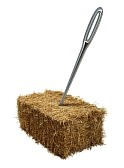
\includegraphics[width=50pt]{imgs/introducao.jpg}
  \label{fig_introducao}
\end{figure}
\end{frame}

%------------------------------------------------

\begin{frame}
\frametitle{Roteiro} % Table of contents slide, comment this block out to remove it
\tableofcontents % Throughout your presentation, if you choose to use \section{} and \subsection{} commands, these will automatically be printed on this slide as an overview of your presentation
\end{frame}

%----------------------------------------------------------------------------------------
%	PRESENTATION SLIDES
%----------------------------------------------------------------------------------------

%------------------------------------------------
\section{Introdução} % Sections can be created in order to organize your presentation into discrete blocks, all sections and subsections are automatically printed in the table of contents as an overview of the talk
%------------------------------------------------

\begin{frame}
\frametitle{Introdução}
\begin{block}{Busca}
 Segundo \citeonline{Sedgewick2011}, sem algoritmos de busca, o desenvolvimento da infra-estrutura computacional que gozamos no mundo moderno não teria sido possível.
\end{block}
\begin{itemize}
\item A busca é uma das funções mais importantes, principalmente em Bancos de Dados;
\item Visa encontrar um registro a partir de uma chave;
\item Neste contexto, utiliza-se o termo {\bf tabela de símbolos} (ou \underline{dicionário}).
\end{itemize}
\end{frame}

%------------------------------------------------

\begin{frame}
\frametitle{Introdução}
\begin{itemize}
\item A tabela de símbolos é um tipo abstrato de dados formado por registros, em que cada registro armazena um {\bf valor} (a informação) e uma {\bf chave} (para busca);
\item A natureza do valor e da chave depende da aplicação;
\item A tabela de símbolos, independente de como é implementada, deve disponibilizar as ações de inserir, buscar e remover registros.
\end{itemize}
\begin{block}{Busca}
 De acordo com \citeonline{Ziviani2011}, a escolha do método de pesquisa mais adequado depende principalmente $(i)$ da quantidade de dados e $(ii)$ da quantidade de operações. 
\end{block}
\end{frame}

%------------------------------------------------

\begin{frame}
\frametitle{Introdução}
\begin{itemize}
\item Diversas estruturas de dados suportam implementar a tabela de símbolos:
  \begin{itemize}
   \item Vetores;
   \item Listas encadeadas;
   \item Árvores (Binária, AVL, Rubro-Negra);
   \item Tabelas {\it hash}.
  \end{itemize}
\item A estrutura de dados utilizada irá definir o método de busca possível.
\end{itemize}
\end{frame}

%------------------------------------------------
\section{Objetivos}
%------------------------------------------------

\begin{frame}
\frametitle{Objetivos}

Esta aula tem como objetivos:

\begin{enumerate}
\item Apresentar os métodos de busca: sequencial e binária;
\item Demonstrar a execução dos algoritmos de busca por meio de exemplos;
\item Analisar o desempenho dos métodos apresentados.
\end{enumerate}

\end{frame}

%------------------------------------------------
\section{Pesquisa Sequencial}
%------------------------------------------------

\begin{frame}
\frametitle{Pesquisa Sequencial}
\begin{itemize}
\item Também chamada de pesquisa exaustiva;
\item É o método de pesquisa mais simples que existe;
\item Utilizado em dados desordenados;
\item Pesquisa sequencialmente do primeiro até o último registro;
  \begin{itemize}
  \item Quando encontrar a chave desejada, para.
  \end{itemize}
\item Formas de implementação:
  \begin{itemize}
  \item Utilizando vetor;
  \item Utilizando lista encadeada.
  \end{itemize}  
\end{itemize}
\end{frame}

%------------------------------------------------

\begin{frame}
\frametitle{Execução Pesquisa Sequencial}
\begin{figure}[!h]
  \centering
  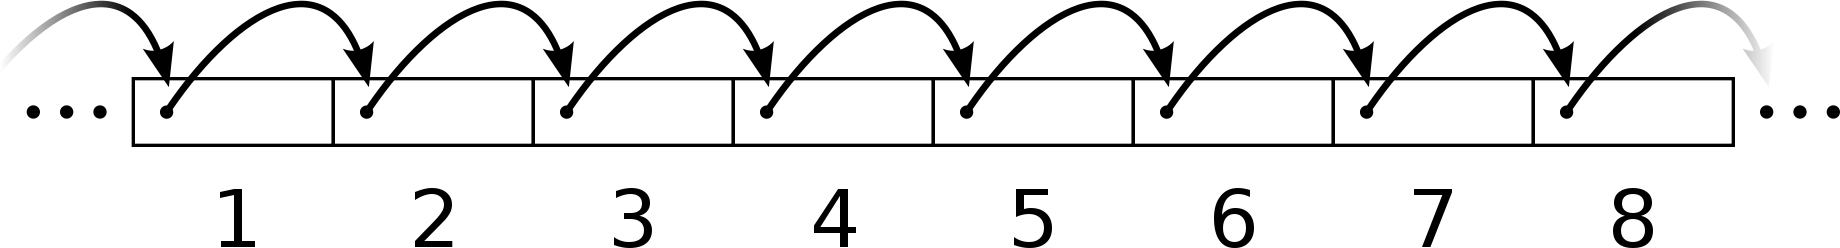
\includegraphics[width=300pt]{imgs/busca_sequencial.png}
  \label{fig_pesquisa_sequencial}
\end{figure}

\end{frame}

%------------------------------------------------

\begin{frame}
\frametitle{Pseudo-código pesquisa sequencial}
\begin{algorithm}[H]
\caption{Pesquisa Sequencial} 
\label{pesquisa_sequencial}
\Entrada{Vetor $V[0..n-1]$ de tamanho $n$, chave $x$ de busca.}
\Saida{Posição $i$ de $x$ em $V$ se $x \in V$ ou $-1$ se $x \notin V$.}
\Inicio{
  \Para{($i \leftarrow 0$ \textrm{ até } $n-1$)} {
    \Se{($x = V[i]$)} {
      \Retorna $i$
    }
  }
  \Retorna $-1$ 
}
\end{algorithm}
\Tiny{Adaptado de \citeonline{Oliveira2011}}
\end{frame}

%------------------------------------------------

\begin{frame}
\frametitle{Pesquisa Sequencial}
\begin{block}{Chaves ordenadas}
 E se as chaves estiverem ordenadas, há melhora?
\end{block}
\pause
   \centering\Large{Sim!} \\
   Ao encontrar um elemento maior que $x$, encerra a busca.
\end{frame}

%------------------------------------------------

\begin{frame}
\frametitle{Pseudo-código pesquisa sequencial (Chaves ordenadas)}
\begin{algorithm}[H]
\caption{Pesquisa Sequencial Ordenada} 
\label{pesquisa_sequencial}
\Entrada{Vetor $V[0..n-1]$ de tamanho $n$ em ordem crescente, chave $x$ de busca.}
\Saida{Posição $i$ de $x$ em $V$ se $x \in V$ ou $-1$ se $x \notin V$.}
\Inicio{
  \Para{($i \leftarrow 0$ \textrm{ até } $n-1$)} {
    \Se{($x = V[i]$)} {
      \Retorna $i$
    }
    \SenaoSe{($V[i] > x$)} {
      \Retorna $-1$
    }
  }
  \Retorna $-1$ 
}
\end{algorithm}
\end{frame}

%------------------------------------------------

\begin{frame}
\frametitle{Pesquisa Sequencial}
Análise da busca sequencial em termos da ordem de crescimento no número de operações:
\begin{itemize}
\item Melhor caso: $1$ operação = $O(1)$;
\item Pior caso: $n$ operações = $O(n)$;
\item Caso médio: $\frac{(n+1)}{2}$ operações = $O(n)$.
\end{itemize}
\end{frame}

%------------------------------------------------

\begin{frame}
\frametitle{Pesquisa Sequencial}
  \begin{block}{Vantagens}
  \begin{itemize}
   \item Codificação simples;
   \item Há melhora de desempenho se os dados buscados com maior frequência forem movidos para o início da sequência;
   \item Dados podem estar desordenados:
      \begin{itemize}
	\item Facilidade na inserção de dados.
      \end{itemize}
  \end{itemize}
  \end{block}
  \begin{block}{Desvantagem}
  Ineficiente para uma quantidade grande de dados.
  \end{block}
\end{frame}


%------------------------------------------------
\section{Pesquisa Binária}
%------------------------------------------------

\begin{frame}
\frametitle{Pesquisa Binária}
\begin{itemize}
\item A pesquisa pode ser muito mais eficiente se os registros forem mantidos em ordem;
\item Nesse caso, compare a chave com a chave do registro que se encontra no meio da tabela:
\begin{itemize}
\item Se a chave é menor, procure na primeira metade da tabela;
\item Se é maior, procure na segunda metade da tabela;
\item Se for igual, a chave foi encontrada;
\item Repita o processo até que a chave seja encontrada ou que reste apenas um elemento.
\end{itemize}
\item A {\bf pesquisa binária} possui esse nome pois, a cada iteração, divide o vetor de busca pela metade;
\item Pode ser implementada apenas utilizando vetores.
\end{itemize}
\end{frame}

%------------------------------------------------

\begin{frame}
\frametitle{Execução Pesquisa Binária}
\begin{figure}[!h]
  \centering
  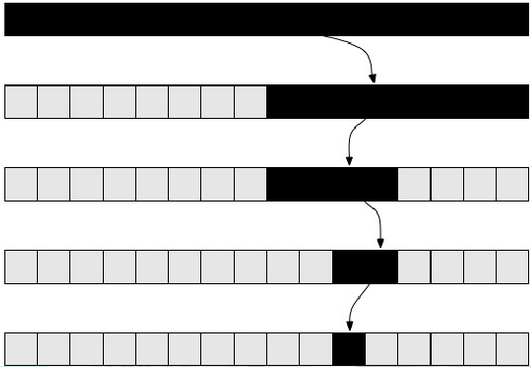
\includegraphics[width=250pt]{imgs/busca_binaria.png}
  \label{fig_busca_binaria}
\end{figure}

\end{frame}

%------------------------------------------------

\begin{frame}
\frametitle{Pseudo-código pesquisa binária (Iterativo)}
\scalebox{0.8}{
\begin{algorithm}[H]
\caption{BuscaBináriaIterativa($V,x,i,f$)} 
\label{pesquisa_binaria_iterativo}
\Entrada{Vetor $V$, chave $x$ de busca, índices inicial $i$ e final $f$ de $V$.}
\Saida{Índice $m$ da posição de $x$ em $V$ ou determina que $x \notin V$.}
\Inicio{
  $encontrado \leftarrow FALSE$ \\
  \Enqto{($i \leq f) \textrm{ AND } (\textrm{ NOT }(encontrado$))}  {
    $m \leftarrow \lfloor \frac{i+f}{2} \rfloor$ \\
    \Se{($V[m] = x$)}{
	$encontrado \leftarrow TRUE$ \\
    }
    \SenaoSe{($x < V[m]$)} {
	$f \leftarrow m - 1$ \\
    } \Senao {
	$i \leftarrow m + 1$ \\
    }    
    
  }
  \Se{($encontrado$)} {
    \Retorna $m$
  } \Senao {
    \Retorna \textrm{``Não encontrado''}
  }
}
\end{algorithm}
}


\Tiny{Adaptado de \citeonline{Feofiloff2015}}
\end{frame}


%------------------------------------------------

\begin{frame}
\frametitle{Pesquisa binária}
\begin{block}{Versão recursiva}
 É possível implementar uma versão mais elegante?
\end{block}
\pause
\centering\Large{Sim!} \\
Utilizando recursão.

\end{frame}

%------------------------------------------------

\begin{frame}
\frametitle{Pseudo-código pesquisa binária (Recursivo)}
\begin{algorithm}[H]
\caption{BuscaBinária($V,x,i,f$)} 
\label{pesquisa_binaria_recursiva}
\Entrada{Vetor $V$, chave $x$ de busca, índices inicial $i$ e final $f$ de $V$.}
\Saida{Índice $i$ da posição de $x$ em $V$ ou determina que $x \notin V$.}
\Inicio{
  \Se{($i = f$)} {
    \Se{($V[i] = x$)} {
	\Retorna i
      } 
      \Senao {
	\Retorna \textrm{``Não encontrado''}
      }
  }
  $m \leftarrow \lfloor \frac{i+f}{2} \rfloor$ \\
  \Se{($V[m] > x$)} {
      \Retorna BuscaBinária($V,x,i,m-1$)      
  }
  \Senao {
      \Retorna BuscaBinária($V,x,m,f$)
  }
}
\end{algorithm}
\Tiny{Adaptado de \citeonline{Oliveira2011}}
\end{frame}


%------------------------------------------------

\begin{frame}
\frametitle{Exemplo Pesquisa Binária}
Procurar o registro com chave = 34.
\begin{figure}[!h]
  \centering
  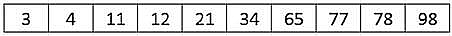
\includegraphics[width=300pt]{imgs/exemplo_busca_binaria1.png}
  \label{fig_exemplo_busca_binaria1}
\end{figure}
\pause
\begin{figure}[!h]
  \centering
  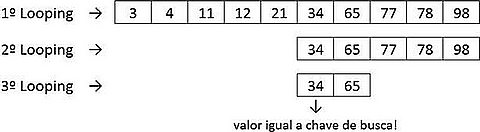
\includegraphics[width=300pt]{imgs/exemplo_busca_binaria2.png}
  \label{fig_exemplo_busca_binaria2}
\end{figure}

\end{frame}

%------------------------------------------------

\begin{frame}
\frametitle{Análise da Pesquisa Binária}
\begin{block} {Versão iterativa}
\begin{itemize}
 \item No melhor caso, $O(1)$;
 \item No caso médio, $O(lg(n))$
 \item No pior caso, $O(lg(n))$;
\end{itemize}
\end{block}
 
\begin{block}{Versão recursiva}
\begin{itemize}
 \item A cada nível de recursão, o tamanho da entrada do problema é dividido por 2;
 \item Não é realizada nenhuma combinação, assim a recorrência é da forma $T(n) = T(\frac{n}{2}) + c$;
 \item Utilizando o método mestre (caso 2), a solução é $\theta(lg(n))$.
\end{itemize}
\end{block}
\end{frame}

%------------------------------------------------

\begin{frame}
\frametitle{Busca Binária}
  \begin{block}{Vantagens}
  \begin{itemize}
   \item Muito mais rápido em relação à pesquisa sequencial;
   \item Simplicidade da implementação;
   \item Caso o registro não seja encontrado, já fornece a posição em que este pode ser inserido.
  \end{itemize}
  \end{block}
  \begin{block}{Desvantagens}
  \begin{itemize}
   \item Só pode ser realizada em vetores;
   \item Os dados devem estar ordenados;
   \item O custo de ordenação é alto ($O(nlogn)$).
  \end{itemize}

  \end{block}
\end{frame}

% 
% %------------------------------------------------
% \section{Tabelas {\it Hash} }
% %------------------------------------------------
% 
% \begin{frame}
% \frametitle{Tabelas {\it Hash}}
% \begin{block}{Tabelas {\it Hash}}
%  Segundo \citeonline{Piva2014}, tabelas {\it hash} (ou \underline{tabelas de dispersão}) consistem no armazenamento de cada elemento em determinado endereço, calculado a paritr da aplicação de uma função sobre a chave de busca.
% \end{block}
% \begin{itemize}
%  \item Matematicamente, teríamos $e = f(c)$, em que $e$ é o endereço, $c$ é a chave de busca, e $f(c)$ é a função que tem como entrada a chave de busca;
%  \item Assim, o processo de pesquisa sobre elementos organizados dessa forma é similar a um acesso direto ao elemento pesquisado.
% \end{itemize}
% 
% \end{frame}
% 
% 
% \begin{frame}
% \frametitle{Tabelas {\it Hash}}
% \begin{itemize}
%  \item A eficiência da pesquisa depende da função de cálculo de endereço $f(c)$;
%  \item A função ideal gera um endereço diferente para cada elemento da tabela (chave de busca);
%  \item Devido a atualizações na tabela, isso é praticamente inviável;
%  \item Uma função possível é $e = c$ mod $n$, em que a função mod corresponde ao resto da divisão inteira de c por $n$, em que $n$ é a quantidade de elementos.
% \end{itemize}
% 
% \end{frame}
% 
% 
% %------------------------------------------------
% 
% \begin{frame}
% \frametitle{Tabelas {\it Hash}}
% \begin{block}{Pesquisa}
%  O processo de pesquisa sobre elementos organizados em uma tabela hash é similar a um acesso direto ao elemento pesquisado.
% \end{block}
% \begin{figure}[!h]
%   \centering
%   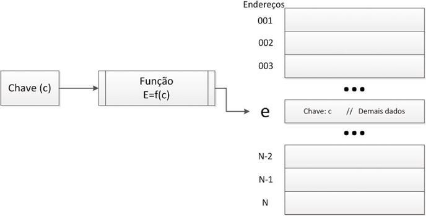
\includegraphics[width=200pt]{imgs/processo_pesquisa.png}
%   \label{fig_processo_pesquisa}
% \end{figure}
% \end{frame}
% 
% %------------------------------------------------
% 
% \begin{frame}
% \frametitle{Exemplo função de dispersão}
% \begin{itemize}
%  \item Tem-se no vetor abaixo, além dos dados, a posição de cada elemento:
% \end{itemize}
% \begin{figure}[!h]
%   \centering
%   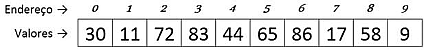
\includegraphics[width=200pt]{imgs/vetor_tabela_hash.png}
%   \label{fig_vetor_tabela_hash}
% \end{figure}
% \pause
% \begin{itemize}
%  \item Numa amostra de dados, aplicando a função de dispersão sugerida, tem-se:
% \end{itemize}
% \begin{figure}[!h]
%   \centering
%   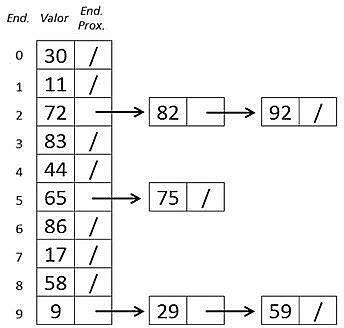
\includegraphics[width=120pt]{imgs/tratamento_colisoes.png}
%   \label{fig_tratamento_colisoes}
% \end{figure}
% \end{frame}
% 
% %------------------------------------------------
% \section{Exercício}
% %------------------------------------------------
% 
% \begin{frame}
% \frametitle{Exercício}
% \begin{block}{Tarefa}
%   \begin{itemize}
%   \item 
%   \end{itemize} 
% \end{block}
% \end{frame}

%------------------------------------------------

\section{Referências bibliográficas}
  \frame{\frametitle{Referências bibliográficas}
    \bibliographystyle{abntex2-alf}
    \bibliography{referencias}
  }

%------------------------------------------------
\begin{frame}
\titlepage % Print the title page as the first slide

\begin{figure}[!h]
  \centering
  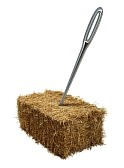
\includegraphics[width=50pt]{imgs/introducao.jpg}
  \label{fig_introducao}
\end{figure}
\end{frame}


%------------------------------------------------

\begin{frame}
\Huge{\centerline{FIM}}

\begin{figure}[!h]
  \centering
  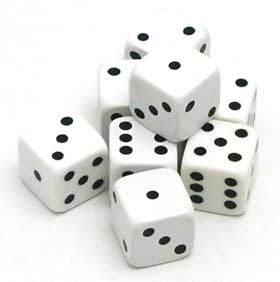
\includegraphics[width=100pt]{imgs/dados.jpg}
  \label{fig_fim}
\end{figure}

\end{frame}

%----------------------------------------------------------------------------------------


\end{document} 